\documentclass{ctexart}
% 此处引入常用包,从此行到46行均无需修改
\usepackage[dvipsnames, svgnames, x11names]{xcolor}
\usepackage{listings}
\usepackage{graphicx}
\usepackage{tabularx}
\usepackage[most]{tcolorbox}
\usepackage{amsmath}
\usepackage{multicol}
\usepackage{multirow}
\usepackage{pifont}
\usepackage{enumitem}
\usepackage{bbding}
\usepackage{colortbl}
\usepackage{placeins}
\usepackage{mathpazo}
\usepackage{bm}
\usepackage{tikz}
\usepackage{xparse}
\usepackage{fancyhdr}
\usepackage[ruled,linesnumbered]{algorithm2e}
\usepackage{algorithmic}

%代码环境设置
\lstset{
    numbers = none ,                                    %可选参数有none,right,left
    breaklines ,                                        %换行有影响,不加这个则换行时从头开始
    numberstyle = \tiny ,                               %数字大小’
    keywordstyle = \color{blue!70} ,                    %关键字颜色
    commentstyle =\color{black!40!white} ,              %注释颜色
    frame = shadowbox ,                                 %阴影设置
    rulesepcolor = \color{red!20!green!20!blue!20} ,    %阴影颜色设置
    escapeinside =`',                                   %lst中文支持不太好,可以用这个括在中文旁边
    basicstyle =\footnotesize\ttfamily                  %代码字体设置
}


%定义题目计数器和命令
\newcounter{questioncnt}
\newcounter{subquestioncnt}[questioncnt]
\newcounter{subsubquestioncnt}[subquestioncnt]

\NewDocumentCommand\question{om}{\noindent\IfNoValueTF{#1}{\textcolor{blue}{\stepcounter{questioncnt}\arabic{questioncnt}}}{#1}\quad#2\par}
\NewDocumentCommand\subquestion{om}{\noindent\IfNoValueTF{#1}{\textcolor{blue}{\stepcounter{subquestioncnt}\arabic{questioncnt}.\arabic{subquestioncnt}}}{#1}\quad#2\par}
\NewDocumentCommand\subsubquestion{om}{\noindent\IfNoValueTF{#1}{\textcolor{blue}{\stepcounter{subsubquestioncnt}\arabic{questioncnt}.\arabic{subquestioncnt}.\arabic{subsubquestioncnt}}}{#1}\quad#2\par}

%定义回答计数器和命令
\newcounter{answercnt}
\newcounter{subanswercnt}[answercnt]
\newcounter{subsubanswercnt}[subanswercnt]

\NewDocumentCommand\answer{o}{\noindent\textcolor{blue}{\IfNoValueTF{#1}{\stepcounter{answercnt}\arabic{answercnt}}{#1}}\quad}
\NewDocumentCommand\subanswer{o}{\noindent\textcolor{blue}{\IfNoValueTF{#1}{\stepcounter{subanswercnt}\arabic{answercnt}.\arabic{subanswercnt}}{#1}}\quad}
\NewDocumentCommand\subsubanswer{o}{\noindent\textcolor{blue}{\IfNoValueTF{#1}{\stepcounter{subsubanswercnt}\arabic{answercnt}.\arabic{subanswercnt}.\arabic{subsubanswercnt}}{#1}}\quad}

%在此处进行基本信息修改
\newcommand{\sCourse}{机器学习}   %课程名
\newcommand{\nTime}{4}             %作业次数
\newcommand{\sName}{黄昊}           %学生姓名
\newcommand{\sNumber}{20204205}     %学号

%页边距设置
\usepackage[left=2cm,right=2cm,top=3cm,bottom=2cm]{geometry}

%页眉页脚设置
\pagestyle{fancy}
\fancyhead[C]{\today}

\newcommand{\homeworkTitle}{
    \setcounter{answercnt}{0}
    %标题部分修改
    \begin{center}
        \fontsize{16pt}{0}{\textbf{\kaishu\sCourse课程\quad第\nTime次作业}}\\
        \fontsize{13pt}{0}{\textit{\kaishu\sName\qquad\sNumber}}\\
    \end{center}}

\begin{document}
\homeworkTitle
选择习题:\answer[4.1]\answer[4.2]\answer[4.3]\answer[4.4]\answer[4.8]

\answer[4.1]
显然成立:构造这样一颗决策树:第一层判断特征向量的第一个分量,第二层判断第二个...
以此类推。由于数据各不相同,故这样构造出来的决策树,必然能分到一个叶节点,且只有一
个数据符合。根据这个构造方法,每个数据到达叶节点的路径各不相同,且一定完全符合(因
为各不冲突),故训练误差为0.

\answer[4.2]
把训练误差作为训练准则容易出现泛化能力差的问题。

\answer[4.3]
\answer[4.4]
代码如下:
\begin{lstlisting}
from math import log
import copy

class DataWrapperAndProcessor:
    def __init__(self,feature,label,feature_title) -> None:
        self.DATA=copy.deepcopy(feature)
        self.LABEL=copy.deepcopy(label)
        self.TITLE=copy.deepcopy(feature_title)
        self.__continousValueProcess()
    
    def entropy(self, dataIdx: list):
        mapping=self.getClassMapping(dataIdx)
        ans = 0
        tot = len(dataIdx)
        for key , val in mapping.items():
            ans += -val / tot * log (val / tot)
        return ans
    
    def entropy_gain(self, dataIdx: list, subsetDataIdx: list):
        totEnt = self.entropy(dataIdx)
        for subIdx in subsetDataIdx:
            totEnt -= len(subIdx) / len(dataIdx) * self.entropy(subIdx)
        return totEnt
    
    def gini(self, dataIdx: list):
        mapping=self.getClassMapping(dataIdx)
        ans = 1
        for key, val in mapping.items():
            ans -= (val / len(dataIdx)) ** 2
        return ans
    
    def gini_ratio(self, dataIdx: list, subsetDataIdx: list):
        gini_tot = 0
        for subIdx in subsetDataIdx:
            gini_tot += self.gini(subIdx) * len(subIdx) / len(dataIdx)
        return gini_tot
    
    def getMaximumClassAndNum(self, dataIdx: list):
        mapping=self.getClassMapping(dataIdx)
        maxVal , label = 0, ""
        for key, val in mapping.items():
            if (val > maxVal):
                label = key
                maxVal = val
        if (label==""):
            return "", 0
        return label, mapping[label]        
    
    def getClassMapping(self, dataIdx: list):       # the class count
        mapping=dict()
        for idx in dataIdx:
            label = self.LABEL[idx]
            mapping[label] = 1 if mapping.get(label) is None else mapping[label] + 1
        return mapping
    
    def getAttrMapping(self, attrIdx: int, dataIdx: list):        # the attr index list
        mapping=dict()
        for idx in dataIdx:
            attrVal = self.DATA[idx][attrIdx]
            mapping[attrVal]=[idx] if mapping.get(attrVal) is None else mapping[attrVal]+[idx]
        return mapping
    
    def __continousValueProcess(self):
        sample = self.DATA[0]
        for idx, val in enumerate(sample):
            if (type(val)==type("str")):
                continue
            else:
                valList = [(self.DATA[i][idx] , i) for i in range(len(self.DATA))]
                valList.sort(key = lambda x : x[0])
                dataIdx = [i for i in range(len(self.DATA))]
                maxentropy_gain = -1
                bestSplit = 0.0
                for i in range(len(valList)-1):             #binary to get the best split point
                    splitPoint = (valList[i][0] + valList[i+1][0]) / 2
                    subListLeft = []
                    subListRight = []
                    for ele in valList:         # create binary subset of data
                        value, index = ele
                        if (value <= splitPoint):
                            subListLeft.append(index)
                        else:
                            subListRight.append(index)
                    entropy_gainVal=self.entropy_gain(dataIdx, [subListLeft,subListRight])
                    if (maxentropy_gain < entropy_gainVal):
                        maxentropy_gain = entropy_gainVal
                        bestSplit = splitPoint
                for sample in self.DATA:
                    val = sample[idx]
                    if (val<=bestSplit):
                        sample[idx] = "<="+str(bestSplit)
                    else:
                        sample[idx] = ">"+str(bestSplit)










class TreeNode:
    def __init__(self , treeDataPraser: DataWrapperAndProcessor, validDataIdx : list = [] ,validAttrIdx : list = []) -> None:
        self.son=[]
        self.criteria=None          # branch tag
        self.criteriaBranch=[]      # branch list corresponding to son
        self.category=None          # class tag in every node
        self.validDataIndex=validDataIdx
        self.validAttrIndex=validAttrIdx
        self.dataParser = treeDataPraser
    
    def isLeaf(self):
        return (len(self.son)==0)

    def nodeSplit(self, optLoss = "entropy"):
        self.category , tot_right_fa= self.dataParser.getMaximumClassAndNum(self.validDataIndex)
        if (tot_right_fa==len(self.validDataIndex) or len(self.validAttrIndex)==0):      # same category or no feature
            return
        bestAttrIdx, maxVal = 0 , 0
        for attrIdx in self.validAttrIndex:
            attrMapping = self.dataParser.getAttrMapping(attrIdx, self.validDataIndex)
            subsetIndex = [lst for _ , lst in attrMapping.items()]
            if (optLoss == "gini"):         # maximunize the value in order to judge
                lossVal = 1 / (self.dataParser.gini_ratio(self.validDataIndex, subsetIndex) + 1e-7)
            else:
                lossVal = self.dataParser.entropy_gain(self.validDataIndex,subsetIndex)
            if (maxVal < lossVal):
                maxVal = lossVal
                bestAttrIdx = attrIdx
        # update this node's result
        self.criteria = self.dataParser.TITLE[bestAttrIdx]
        attrMapping = self.dataParser.getAttrMapping(bestAttrIdx, self.validDataIndex)
        tot_right_sub = 0
        for attrVal, subsetIdx in attrMapping.items():  #spawn son node
            attrIdxList = copy.deepcopy(self.validAttrIndex)
            attrIdxList.remove(bestAttrIdx)
            node = TreeNode(self.dataParser, subsetIdx, attrIdxList)
            node.category , num = self.dataParser.getMaximumClassAndNum(subsetIdx)
            # print(num)
            tot_right_sub += num
            self.son.append(node)
            self.criteriaBranch.append(attrVal)
    










class DecisionTree:
    def __init__(self,dataPraser: DataWrapperAndProcessor):
        self.dataPraser=dataPraser
        self.root=TreeNode(self.dataPraser,[i for i in range(len(dataPraser.DATA))],[i for i in range(len(dataPraser.TITLE))])
        
    def buildTree(self, node: TreeNode, optLoss="entropy"):
        node.nodeSplit(optLoss=optLoss)
        for son in node.son:
            self.buildTree(son, optLoss)
    
    def post_prun(self, node: TreeNode, dataPraser: DataWrapperAndProcessor):
        if (node.isLeaf()==True):
            attr, tot_right = dataPraser.getMaximumClassAndNum(node.validDataIndex)
            if (attr == node.category):
                return tot_right
            else: 
                return 0
        tot_right_son = 0
        for son in node.son:
            tot_right_son += self.post_prun(son,dataPraser)
        attr, tot_right_fa = dataPraser.getMaximumClassAndNum(node.validDataIndex)
        # print(tot_right_fa,tot_right_son,node.criteriaBranch,node.criteria)
        if (tot_right_fa > tot_right_son):
            node.son = []
            node.category = attr
            return tot_right_fa
        elif (tot_right_fa == tot_right_son):
            mapping={}
            for son in node.son:
                cat = son.category
                mapping[cat] = 1 if mapping.get(cat) is None else mapping[cat]+1
            if (len(mapping)==1):       # prun
                node.son = []
                node.category = attr
        return tot_right_son

    def pre_prun(self, node: TreeNode, dataPraser: DataWrapperAndProcessor):
        if (node.isLeaf()==True):
            attr, tot_right = dataPraser.getMaximumClassAndNum(node.validDataIndex)
            if (attr == node.category):
                return tot_right
            else: 
                return 0
        tot_right_son = 0
        for son in node.son:
            attr , num = dataPraser.getMaximumClassAndNum(son.validDataIndex)
            tot_right_son += num
        attr, tot_right_fa = dataPraser.getMaximumClassAndNum(node.validDataIndex)
        if (tot_right_fa >= tot_right_son):
            # print(node.criteriaBranch,node.criteria)
            node.son = []
            node.category = attr
        for son in node.son:
            self.pre_prun(son, dataPraser)
        return tot_right_son
    
    def printTree(self,node: TreeNode, layer = 1, seq = 1):
        if (node.isLeaf()==True):
            print("`第' {} `层,第' {} `个【叶子】的信息:'\n\t`分类类别:'{}".format(layer, seq, node.category))
        else:
            print("`第' {} `层,第' {} `个【节点】的信息:'\n\t`分类属性:'{}\n\t`子节点分支内容:'{}\n\t`子节点所含样本:'{}\n\t`分类类别:'{}".format(layer, seq, node.criteria, node.criteriaBranch,[son.validDataIndex for son in node.son],node.category))
        for idx, son in enumerate(node.son):
            self.printTree(son, layer+1, idx+1)

    def __predict(self, idx , sample, title, node : TreeNode):
        node.validDataIndex.append(idx)
        if node.isLeaf()==True:
            return node.category
        attrIdx = 0
        for idx_attr, attr in enumerate(title):
            if attr==node.criteria:
                attrIdx = idx_attr
                break
        for idx_son, cat in enumerate(node.criteriaBranch):
            if sample[attrIdx] == cat:
                return self.__predict(idx , sample, title, node.son[idx_son])
    
    def tagClean(self, node: TreeNode):
         node.validDataIndex = []
         for son in node.son:
             self.tagClean(son)
    
    def tagWithData(self,node:TreeNode, dataPraser:DataWrapperAndProcessor):
        for idx, sample in enumerate(dataPraser.DATA):
            pred = self.__predict(idx , sample, dataPraser.TITLE, self.root)
    
    def reTag(self, node:TreeNode,dataPraser:DataWrapperAndProcessor):
        self.tagClean(node)
        self.tagWithData(node,dataPraser)
    
    def getAccuracy(self, dataPraser: DataWrapperAndProcessor):     # give tag and get accuracy
        self.tagClean(self.root)
        ans = 0
        rightSet = []
        wrongSet = []
        tot = len(dataPraser.LABEL)
        for idx, sample in enumerate(dataPraser.DATA):
            pred = self.__predict(idx , sample, dataPraser.TITLE, self.root)
            if pred == dataPraser.LABEL[idx]:
                ans += 1
                rightSet.append(idx)
            else:
                wrongSet.append(idx)
        return ans/tot , rightSet , wrongSet
    
    def printAcc(self, dataPraser: DataWrapperAndProcessor):
        acc, _, _=self.getAccuracy(dataPraser)
        print("`准确率为:'{}%".format(acc * 100))

# 4.3
feature=[["`青绿","蜷缩","浊响","清晰","凹陷","硬滑"',0.697,0.46],
[`"乌黑","蜷缩","沉闷","清晰","凹陷","硬滑",'0.774,0.376],
[`"乌黑","蜷缩","浊响","清晰","凹陷","硬滑",'0.634,0.264],
[`"青绿","蜷缩","沉闷","清晰","凹陷","硬滑",'0.608,0.318],
[`"浅白","蜷缩","浊响","清晰","凹陷","硬滑",'0.556,0.215],
[`"青绿","稍蜷","浊响","清晰","稍凹","软粘",'0.403,0.237],
[`"乌黑","稍蜷","浊响","稍糊","稍凹","软粘",'0.481,0.149],
[`"乌黑","稍蜷","浊响","清晰","稍凹","硬滑",'0.437,0.211],
[`"乌黑","稍蜷","沉闷","稍糊","稍凹","硬滑",'0.666,0.091],
[`"青绿","硬挺","清脆","清晰","平坦","软粘",'0.243,0.267],
[`"浅白","硬挺","清脆","模糊","平坦","硬滑",'0.245,0.057],
[`"浅白","蜷缩","浊响","模糊","平坦","软粘",'0.343,0.099],
[`"青绿","稍蜷","浊响","稍糊","凹陷","硬滑",'0.639,0.161],
[`"浅白","稍蜷","沉闷","稍糊","凹陷","硬滑",'0.657,0.198],
[`"乌黑","稍蜷","浊响","清晰","稍凹","软粘",'0.36,0.37],
[`"浅白","蜷缩","浊响","模糊","平坦","硬滑",'0.593,0.042],
[`"青绿","蜷缩","沉闷","稍糊","稍凹","硬滑",'0.719,0.103]]
label=[1,1,1,1,1,1,1,1,0,0,0,0,0,0,0,0,0]
feature_title=[`"色泽","根蒂","敲声","纹理","脐部","触感","密度","含糖率'"]
print("========4.3========")
dataPraser_1=DataWrapperAndProcessor(feature,label,feature_title)
model=DecisionTree(dataPraser_1)
model.buildTree(model.root)
model.printTree(model.root)
model.printAcc(dataPraser_1)

# 4.4
feature_train=[["`青绿","蜷缩","浊响","清晰","凹陷","硬滑'"],
["`乌黑","蜷缩","沉闷","清晰","凹陷","硬滑"'],
["`乌黑","蜷缩","浊响","清晰","凹陷","硬滑"'],
["`青绿","稍蜷","浊响","清晰","稍凹","软粘"'],
["`乌黑","稍蜷","浊响","稍糊","稍凹","软粘"'],
["`青绿","硬挺","清脆","清晰","平坦","软粘"'],
["`浅白","稍蜷","沉闷","稍糊","凹陷","硬滑"'],
["`乌黑","稍蜷","浊响","清晰","稍凹","软粘"'],
["`浅白","蜷缩","浊响","模糊","平坦","硬滑"'],
["`青绿","蜷缩","沉闷","稍糊","稍凹","硬滑"']]

feature_test=[["`青绿","蜷缩","沉闷","清晰","凹陷","硬滑'"],
["`浅白","蜷缩","浊响","清晰","凹陷","硬滑'"],
["`乌黑","稍蜷","浊响","清晰","稍凹","硬滑'"],
["`乌黑","稍蜷","沉闷","稍糊","稍凹","硬滑'"],
["`浅白","硬挺","清脆","模糊","平坦","硬滑'"],
["`浅白","蜷缩","浊响","模糊","平坦","软粘'"],
["`青绿","稍蜷","浊响","稍糊","凹陷","硬滑'"],]
label_train=[1,1,1,1,1,0,0,0,0,0]
label_test=[1,1,1,0,0,0,0]
feature_title=["`色泽","根蒂","敲声","纹理","脐部","触感'"]
print("========4.4========")
dataPraser_train=DataWrapperAndProcessor(feature_train,label_train,feature_title)
dataPraser_test=DataWrapperAndProcessor(feature_test,label_test,feature_title)
# origin
optLoss="gini"
print("origin tree")
model=DecisionTree(dataPraser_train)
model.buildTree(model.root, optLoss=optLoss)
model.printTree(model.root)
model.printAcc(dataPraser_test)
# pre prunning
print("pre prunning")
model=DecisionTree(dataPraser_train)
model.buildTree(model.root, optLoss=optLoss)
model.reTag(model.root, dataPraser_test)
model.pre_prun(model.root, dataPraser_test)
model.printTree(model.root)
model.printAcc(dataPraser_test)
# post prunning
print("post prunning")
model=DecisionTree(dataPraser_train)
model.buildTree(model.root, optLoss=optLoss)
model.reTag(model.root, dataPraser_test)
model.post_prun(model.root, dataPraser_test)
model.printTree(model.root)
model.printAcc(dataPraser_test)
\end{lstlisting}
程序执行结果为(绘制的决策树在程序执行结果后面):
\begin{tcolorbox}[colframe = blue, colback = blue!10!white ,  breakable]
========4.3========\newline
第 1 层,第 1 个【节点】的信息:\newline
        分类属性:纹理\newline
        子节点分支内容:['清晰', '稍糊', '模糊']\newline
        子节点所含样本:[[0, 1, 2, 3, 4, 5, 7, 9, 14], [6, 8, 12, 13, 16], [10, 11, 15]]\newline
        分类类别:0\newline
第 2 层,第 1 个【节点】的信息:\newline
        分类属性:密度\newline
        子节点分支内容:['>0.3815', '<=0.3815']\newline
        子节点所含样本:[[0, 1, 2, 3, 4, 5, 7], [9, 14]]\newline
        分类类别:1\newline
第 3 层,第 1 个【叶子】的信息:\newline
        分类类别:1\newline
第 3 层,第 2 个【叶子】的信息:\newline
        分类类别:0\newline
第 2 层,第 2 个【节点】的信息:\newline
        分类属性:触感\newline
        子节点分支内容:['软粘', '硬滑']\newline
        子节点所含样本:[[6], [8, 12, 13, 16]]\newline
        分类类别:0\newline
第 3 层,第 1 个【叶子】的信息:\newline
        分类类别:1\newline
第 3 层,第 2 个【叶子】的信息:\newline
        分类类别:0\newline
第 2 层,第 3 个【叶子】的信息:\newline
        分类类别:0\newline
准确率为:100.0\%\newline
========4.4========\newline
origin tree\newline
第 1 层,第 1 个【节点】的信息:\newline
        分类属性:色泽\newline
        子节点分支内容:['青绿', '乌黑', '浅白']\newline
        子节点所含样本:[[0, 3, 5, 9], [1, 2, 4, 7], [6, 8]]\newline
        分类类别:1\newline
第 2 层,第 1 个【节点】的信息:\newline
        分类属性:敲声\newline
        子节点分支内容:['浊响', '清脆', '沉闷']\newline
        子节点所含样本:[[0, 3], [5], [9]]\newline
        分类类别:1\newline
第 3 层,第 1 个【叶子】的信息:\newline
        分类类别:1\newline
第 3 层,第 2 个【叶子】的信息:\newline
        分类类别:0\newline
第 3 层,第 3 个【叶子】的信息:\newline
        分类类别:0\newline
第 2 层,第 2 个【节点】的信息:\newline
        分类属性:根蒂\newline
        子节点分支内容:['蜷缩', '稍蜷']\newline
        子节点所含样本:[[1, 2], [4, 7]]\newline
        分类类别:1\newline
第 3 层,第 1 个【叶子】的信息:\newline
        分类类别:1\newline
第 3 层,第 2 个【节点】的信息:\newline
        分类属性:纹理\newline
        子节点分支内容:['稍糊', '清晰']\newline
        子节点所含样本:[[4], [7]]\newline
        分类类别:1\newline
第 4 层,第 1 个【叶子】的信息:\newline
        分类类别:1\newline
第 4 层,第 2 个【叶子】的信息:\newline
        分类类别:0\newline
第 2 层,第 3 个【叶子】的信息:\newline
        分类类别:0\newline
准确率为:28.57142857142857\%\newline
pre prunning\newline
第 1 层,第 1 个【叶子】的信息:\newline
        分类类别:0\newline
准确率为:57.14285714285714\%\newline
post prunning\newline
第 1 层,第 1 个【节点】的信息:\newline
        分类属性:色泽\newline
        子节点分支内容:['青绿', '乌黑', '浅白']\newline
        子节点所含样本:[[0, 6], [2, 3], [1, 4, 5]]\newline
        分类类别:1\newline
第 2 层,第 1 个【叶子】的信息:\newline
        分类类别:1\newline
第 2 层,第 2 个【叶子】的信息:\newline
        分类类别:1\newline
第 2 层,第 3 个【叶子】的信息:\newline
        分类类别:0\newline
准确率为:57.14285714285714\%\newline
\end{tcolorbox}
所对应的决策树为:

\begin{figure}[htbp]
    \centering
    \label{fig:4.3}
    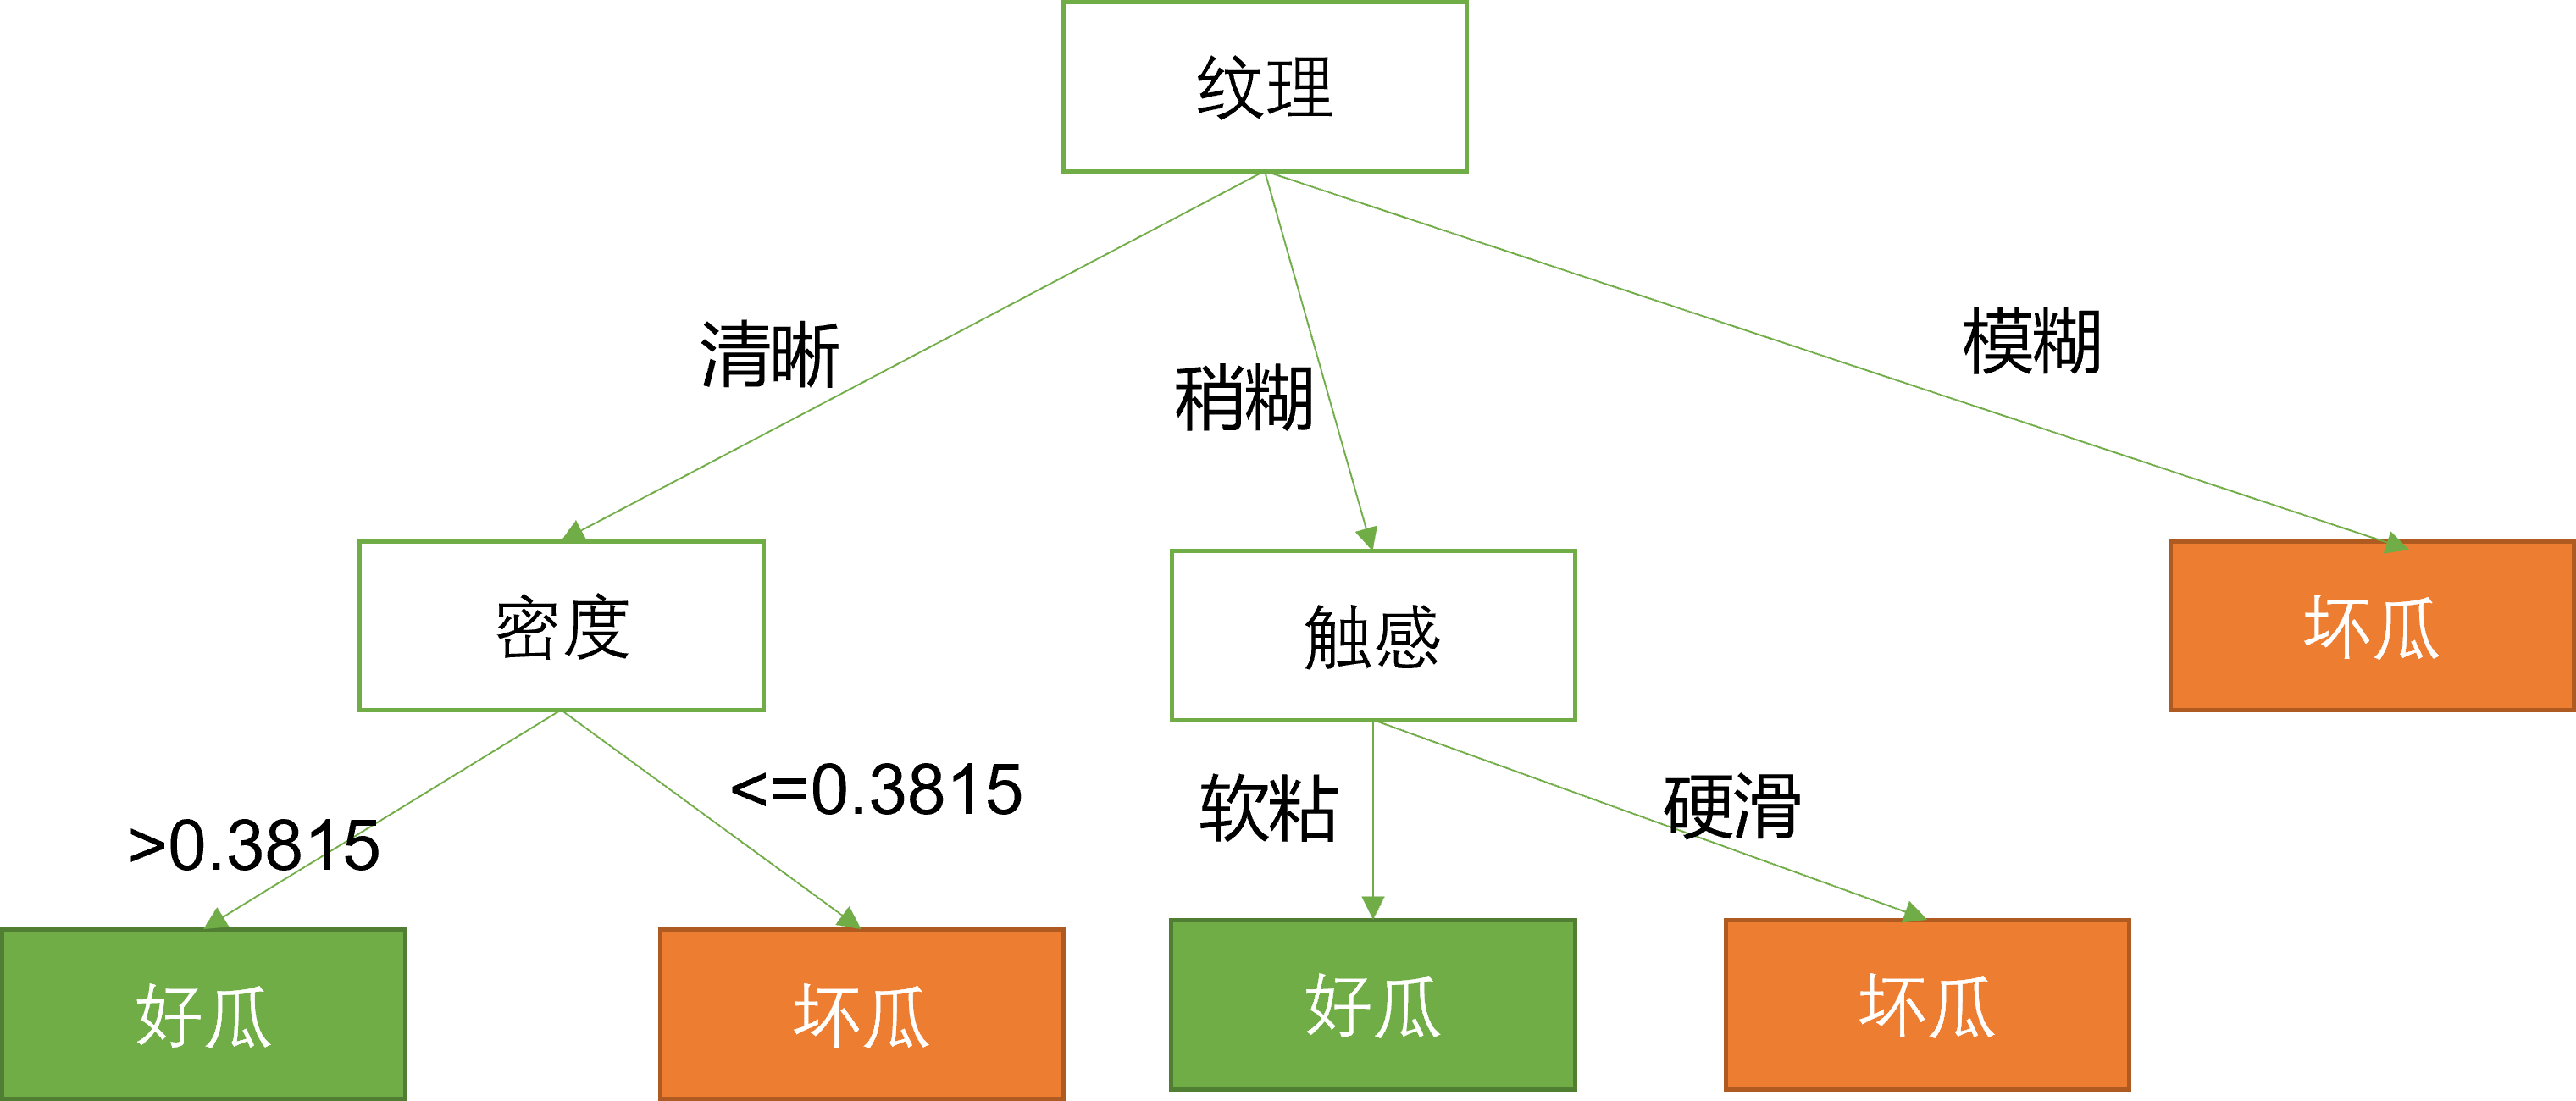
\includegraphics[scale=.5]{images/4.3.png}
    \caption{4.3的决策树}
\end{figure}


\begin{figure}[htbp]
    \centering
    \label{fig:4.4.1}
    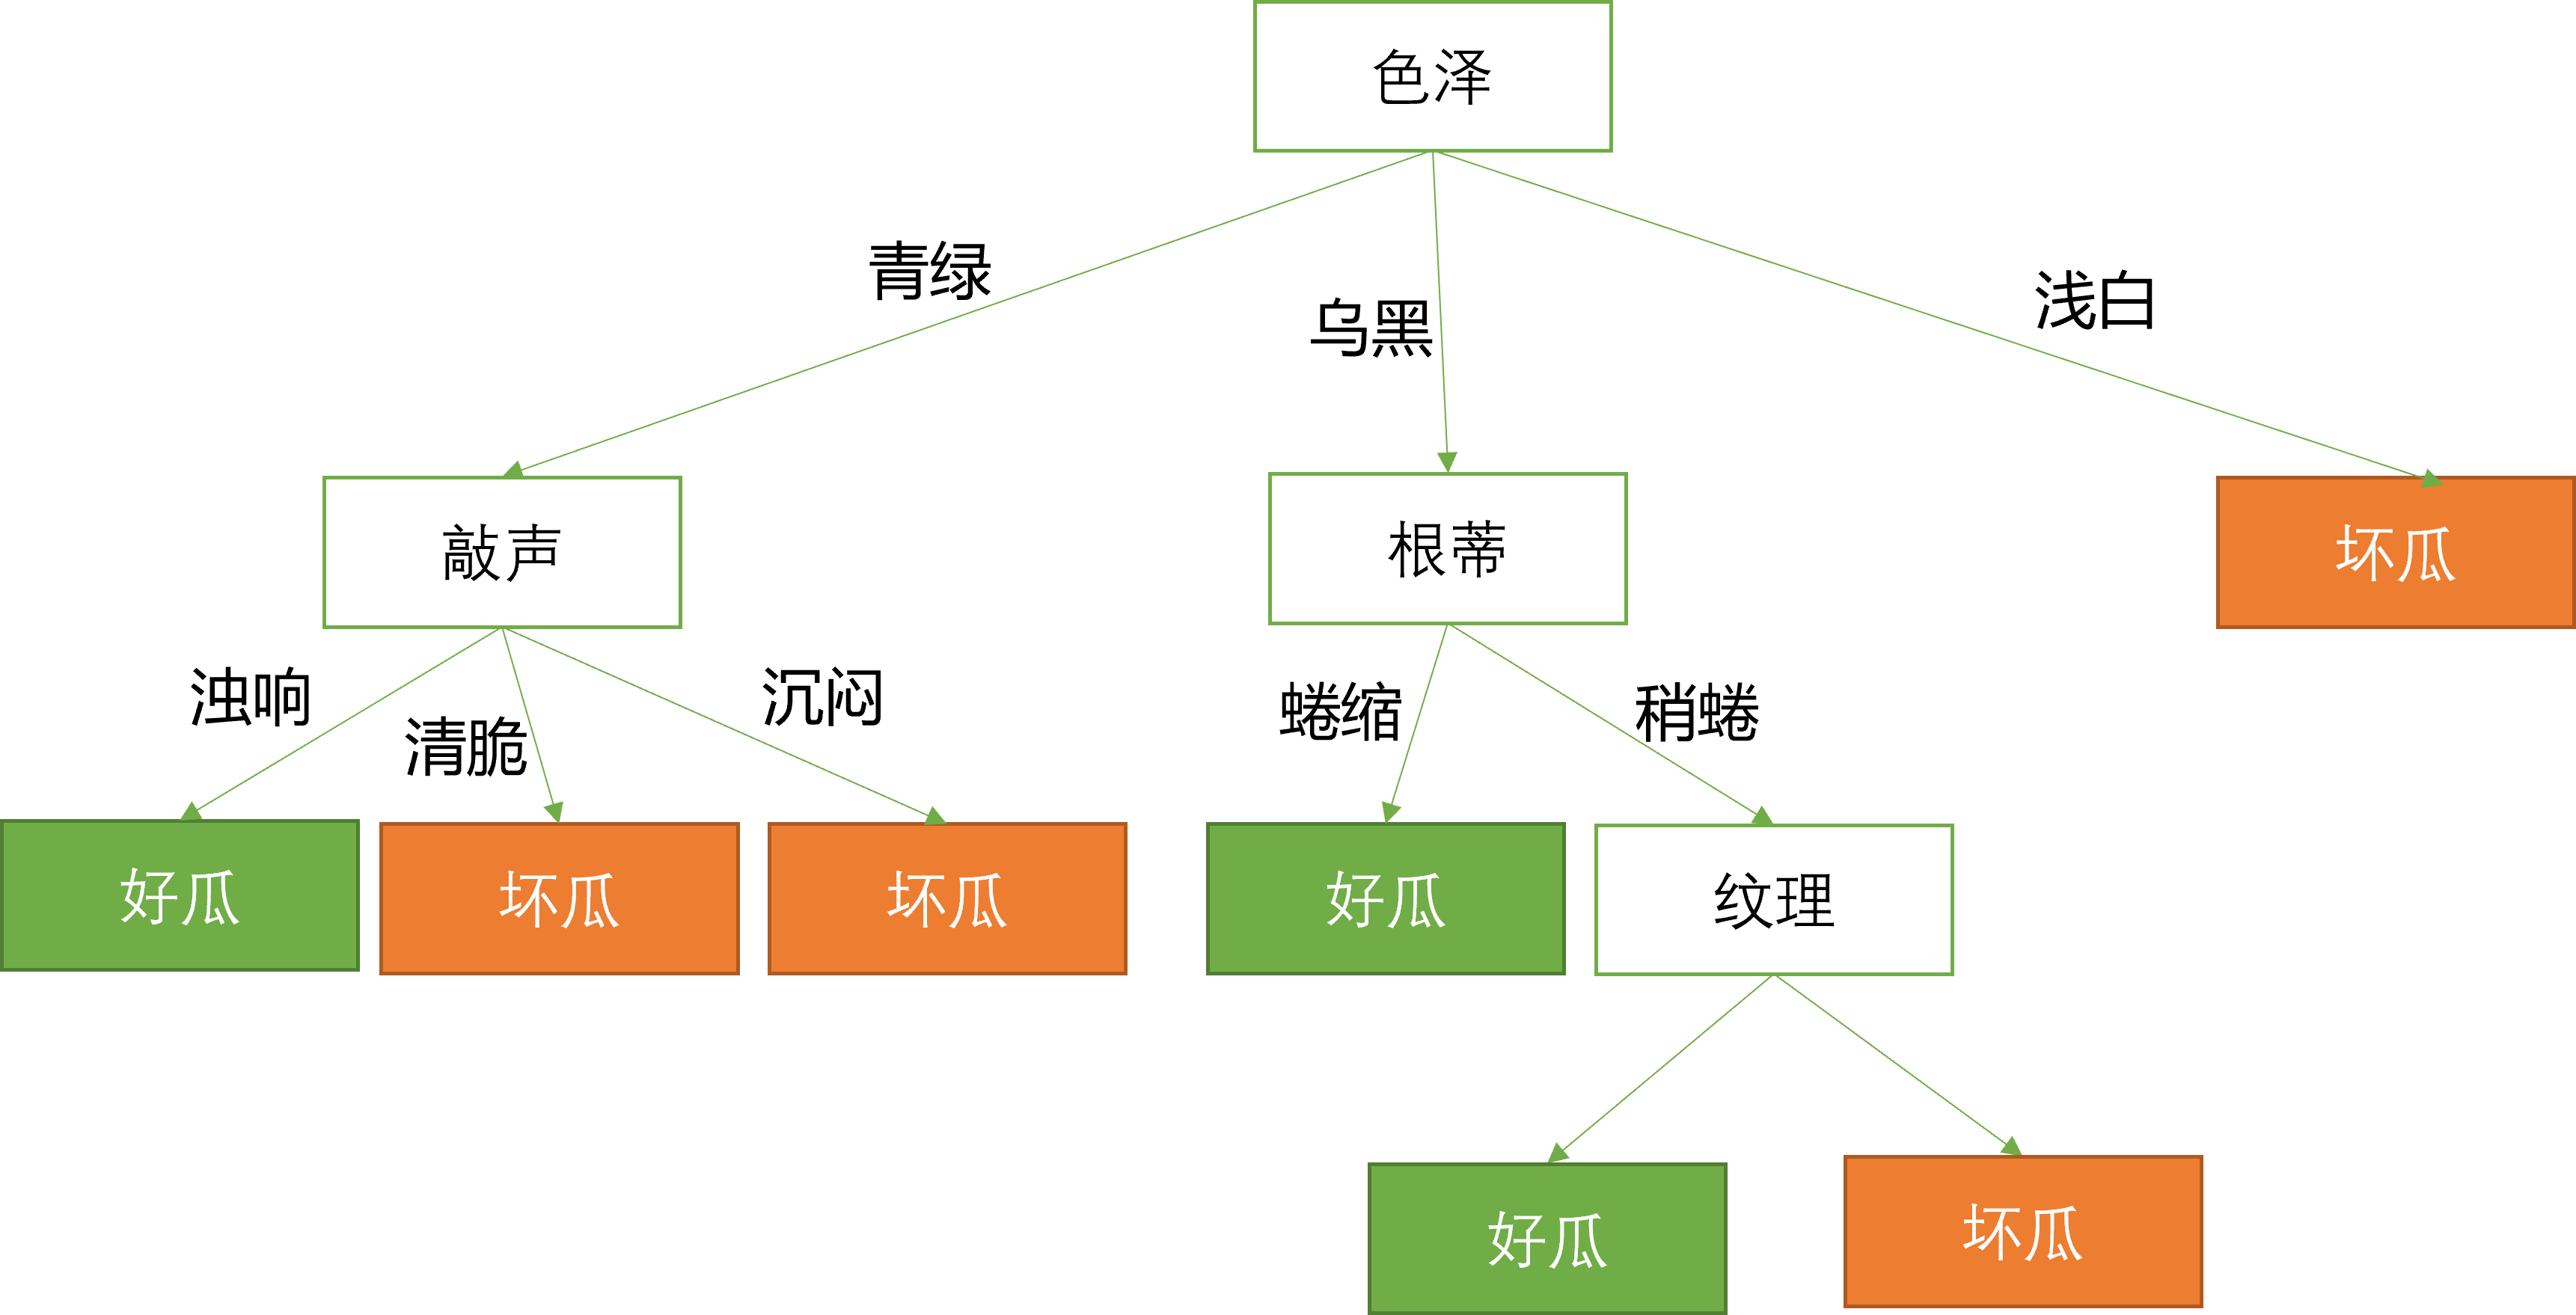
\includegraphics[scale=.5]{images/4.4.1.png}
    \caption{4.4的原始决策树}
\end{figure}


\begin{figure}[htbp]
    \centering
    \label{fig:4.4.2}
    
\includegraphics[scale=1]{images/4.4.2.png}
    \caption{4.4进行预剪枝的决策树}
\end{figure}


\begin{figure}[htbp]
    \centering
    \label{fig:4.4.3}
    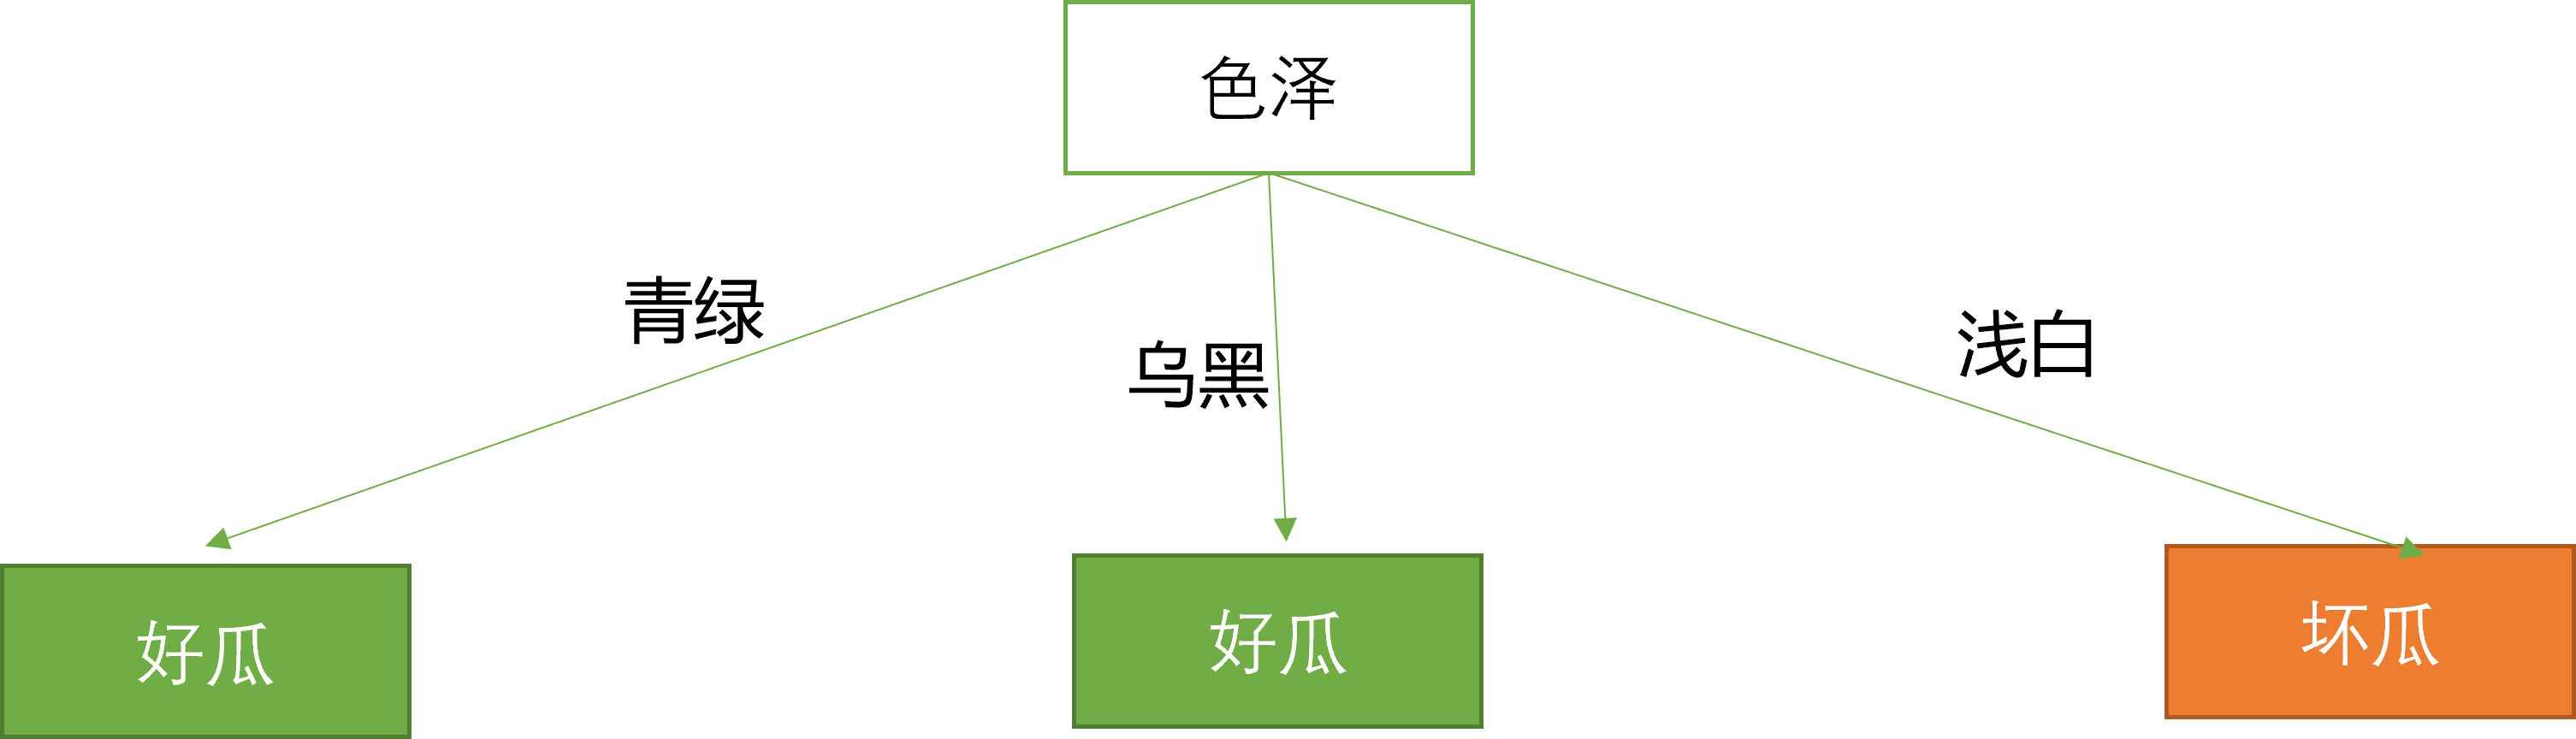
\includegraphics[scale=.8]{images/4.4.3.png}
    \caption{4.4进行后剪枝的决策树}
\end{figure}
\newpage
4.4问的决策树,对于预剪枝的决策树,仅剩下树根,训练集有7个样本,4个坏瓜,准确率为57.14\%;后剪枝的决策树,
有两个坏瓜和两个好瓜分别预测正确,准确率也为57.14\%。而对比于原始的决策树,在训练集上的准确率仅为28.57\%,结果
有所提升,但预剪枝形成的决策树,由于数据量少,很可能有欠拟合的风险。相比之下,后剪枝生成的决策树较为合理。

\answer[4.8]
如果属性取值较多但属性少,BFS比DFS空间消耗更大;若属性多但属性值少,则DFS比BFS空间消耗更大,DFS有爆栈的风险。
\begin{algorithm}
\caption{决策树生成算法——基于广度优先搜索}\label{algorithm}
\KwData{训练集D=\{$(x_1,y_1),(x_2,y_2),\dots,(x_m,y_m)$\}\\\qquad\ \ \ 属性集A=\{$a_1,a_2,\dots,a_d$\}\\\qquad\ \ \ 最大高度 MaxDepth}
\KwResult{决策树$T$}
生成节点$N$,节点信息包括数据集$D$,属性集$A$,高度信息$h$;\\
记录决策树T的根为N;\\
生成节点队列Q;\\
将N压入队列Q的队尾;\\
\While{节点队列Q非空}{
    从节点队列Q中取出队首节点N;\\
    \If{节点N.D中样本全属于同一类别C}{将N标记为C类叶节点;\textbf{continue};}
    \If{节点N.h已达到MaxDepth \textbf{OR} $N.A=\emptyset$ \textbf{OR} N.D中样本在N.A上的取值相同}{将N标记为叶节点,其类别标记为N.D中样本最多的类;\textbf{continue};}
    从N.A中选择最优划分属性$a_*$;\\
    \For{$a_*$的每一个值$a_*^v$}{
        为N生成一个分支;令$D_v$为D中在$a_*$上取值为$a_*^v$的样本子集;\\
        \eIf{$D_v$为空}
        {将分支节点标记为叶节点,其类别表及为D中样本最多的类;continue;}
        {生成节点$N_s$,节点信息包括数据集$D_v$,属性集$A$\textbackslash$\{a_*\}$,高度信息$N.h+1$;\\将$N_s$压入节点队列Q}
    }
}
\textbf{return} 决策树T
\end{algorithm}

\end{document}